\documentclass[12pt,a4paper]{article}

%%%%%%%%%%%%%%%%%%%%%%%%%%%%%%%%%%
% Encoding and language
\usepackage[utf8]{inputenc}
\usepackage[T1]{fontenc}
\usepackage[english]{babel}
\selectlanguage{English}

%%%%%%%%%%%%%%%%%%%%%%%%%%%%%%%%%%
% General packages
\usepackage{verbatim}
\usepackage[all]{xy}
\usepackage{float}
\usepackage{amsmath}
\usepackage{array}
\usepackage{listings}
\usepackage{xcolor}
\usepackage{setspace}
\usepackage{booktabs}
\usepackage{graphicx}
\usepackage{url}
\usepackage{lmodern}
\interfootnotelinepenalty=10000

%%%%%%%%%%%%%%%%%%%%%%%%%%%%%%%%%%
% Page layout
\usepackage{geometry}
\geometry{margin=2.5cm}

%%%%%%%%%%%%%%%%%%%%%%%%%%%%%%%%%%
% Hyperlinks
\usepackage[
    colorlinks=true,
    urlcolor=blue!50!black,
    linkcolor=black,
    citecolor=black
]{hyperref}

%%%%%%%%%%%%%%%%%%%%%%%%%%%%%%%%%%
% Bibliography
\usepackage[round]{natbib}

%%%%%%%%%%%%%%%%%%%%%%%%%%%%%%%%%%
% Fancy headers (ALL pages incl. title page)
\usepackage{fancyhdr}
\pagestyle{fancy}

\fancyhf{} % clear header/footer

\fancyhead[L]{zpn710, fps618, kvb125, xnc401 - everyone contributed equally}
\fancyhead[R]{February 2026}
\fancyfoot[C]{\thepage}

\renewcommand{\headrulewidth}{0.4pt}
\renewcommand{\footrulewidth}{0pt}

% IMPORTANT: make 'plain' style match 'fancy'
\fancypagestyle{plain}{
    \fancyhf{}
    \fancyhead[L]{zpn710, fps618, kvb125, xnc401 - everyone contributed equally}
    \fancyhead[R]{February 2026}
    \fancyfoot[C]{\thepage}
    \renewcommand{\headrulewidth}{0.4pt}
}

%%%%%%%%%%%%%%%%%%%%%%%%%%%%%%%%%%
% Listings styles
\lstdefinestyle{CStyle}{
    language=C,
    basicstyle=\small\ttfamily,
    keywordstyle=\color{blue},
    commentstyle=\color{green!40!black},
    stringstyle=\color{orange},
    numbers=left,
    numberstyle=\tiny,
    stepnumber=1,
    numbersep=5pt,
    backgroundcolor=\color{gray!5},
    frame=single,
    rulecolor=\color{black!30},
    captionpos=b,
    breaklines=true,
    breakatwhitespace=true,
    tabsize=4,
    showspaces=false,
    showstringspaces=false,
}

\definecolor{bluekeywords}{rgb}{0.13,0.13,1}
\definecolor{greencomments}{rgb}{0,0.5,0}
\definecolor{turqusnumbers}{rgb}{0.17,0.57,0.69}
\definecolor{redstrings}{rgb}{0.5,0,0}

\lstdefinelanguage{FSharp}{
    morekeywords={let,new,match,with,rec,open,module,namespace,type,of,member,and,for,in,do,begin,end,fun,function,try,mutable,if,then,else},
    keywordstyle=\color{bluekeywords},
    sensitive=false,
    morecomment=[l][\color{greencomments}]{///},
    morecomment=[l][\color{greencomments}]{//},
    morecomment=[s][\color{greencomments}]{{(*}{*)}},
    morestring=[b]",
    stringstyle=\color{redstrings}
}

%%%%%%%%%%%%%%%%%%%%%%%%%%%%%%%%%%
% Matrix spacing fix
\makeatletter
\renewcommand*\env@matrix[1][*\c@MaxMatrixCols c]{%
  \hskip -\arraycolsep
  \let\@ifnextchar\new@ifnextchar
  \array{#1}}
\makeatother

%%%%%%%%%%%%%%%%%%%%%%%%%%%%%%%%%%
% Graphics paths
\graphicspath{{figures/}{anotherFigureDirectory/}}

%%%%%%%%%%%%%%%%%%%%%%%%%%%%%%%%%%
% Title (no author/date under title)
\title{\LARGE \textbf{Handin 1 Numerical Optimization} \\[1ex]}
\date{}

\makeatletter
\def\@maketitle{%
  \newpage
  \null
  \vskip 1em % ← space above title (adjust if you want)
  \begin{center}%
    {\LARGE \bfseries \@title \par}%
    \vskip 0.5em % ← space below title (THIS controls the gap)
  \end{center}%
}
\makeatother

%%%%%%%%%%%%%%%%%%%%%%%%%%%%%%%%%%
\begin{document}

\maketitle

\section{Introduction}

This report investigates several quasi-Newton and Newton-type methods through both theoretical analysis and systematic experiments on benchmark test functions. We assess both convergence efficiency and also robustness and reliability.

\section{Theoretical Assignment}

\paragraph{Method}
We analyze the transformed ellipsoid function $f_3$ in one dimension ($d=1$). 
Since the Hessian of a scalar function in $d=1$ equals its second derivative, positive definiteness is equivalent to $f_3''(x)>0$.

\paragraph{Function definition}
For $d=1$ and $\alpha^{0/0}=1$, the ellipsoid function is $f_1(x)=x^2$. 
So,
\[
f_3(x)=\frac{f_1(x)}{\varepsilon+f_1(x)}=\frac{x^2}{\varepsilon+x^2}, \qquad \varepsilon>0
\]

\paragraph{First derivative}

\[
f_3'(x)=\frac{2x(\varepsilon+x^2)-x^2(2x)}{(\varepsilon+x^2)^2}
       =\frac{2\varepsilon x}{(\varepsilon+x^2)^2}
\]

\paragraph{Second derivative}

\[
f_3''(x)
=\frac{2\varepsilon(\varepsilon+x^2)^2-2\varepsilon x\cdot2(\varepsilon+x^2)(2x)}{(\varepsilon+x^2)^4}
=\frac{2\varepsilon(\varepsilon+x^2)(\varepsilon-3x^2)}{(\varepsilon+x^2)^4}
=\frac{2\varepsilon(\varepsilon-3x^2)}{(\varepsilon+x^2)^3}
\]

\paragraph{Positive definiteness}
Since $\varepsilon>0$ and $(\varepsilon+x^2)^3>0$ for all $x$, the sign of $f_3''(x)$ is determined by $\varepsilon-3x^2$ and
\[
f_3''(x)>0
\;\Longleftrightarrow\;
\varepsilon-3x^2>0
\;\Longleftrightarrow\;
|x|<\sqrt{\frac{\varepsilon}{3}}
\]

\paragraph{Conclusion}
The Hessian of $f_3$ is positive definite, and $f_3$ is locally convex for
\[
|x|<\sqrt{\frac{\varepsilon}{3}}
\]

\section{Programming Assignment}

\subsection{Testing Protocol}
All algorithms are evaluated under identical experimental conditions to ensure a fair comparison. 
For each test function, multiple random initial points are sampled, and all algorithms are initialised from the same points. This is to analyses sensitivity/robustness to starting points. We sampled 100 initial points from multivariate Gaussian $\text{N}(x^*,100 \cdot \text{I})$ centered at each function's optimum. This was simply a choice we made. We do not have a prior and therefore we have a large variance. We also considered using a normal distribution around 0 to remove information leak.

Each algorithm is run until convergence or until a maximum number of iterations is reached. 
Convergence requires the norm of the gradient to fall below a fixed tolerance~$\varepsilon = 10^{-8}$.
Runs that do not satisfy this criteria are unsuccessful.

\subsection{Experimental Results and Robustness}

For each algorithm, we have plotted the median convergence trajectory over multiple random initialisations is shown, together with a shaded region representing the range 50th to 75th percentile. This is shown in Figure ~\ref{fig:convergence}.
The 99th percentile is additionally included to capture rare but extreme convergence behavior. The y-axis is cut to the tolerance $\varepsilon=10^{-8}$. We chose to use median instead of average because it is more robust from outliers and we don't know how we should take the average after some trajectories have reached the threshold.
We look at the 75th and 99th percentile because we mainly care about how well we can expect the algorithms to work in the worst case or average case.

\begin{figure}[H]
    \centering
    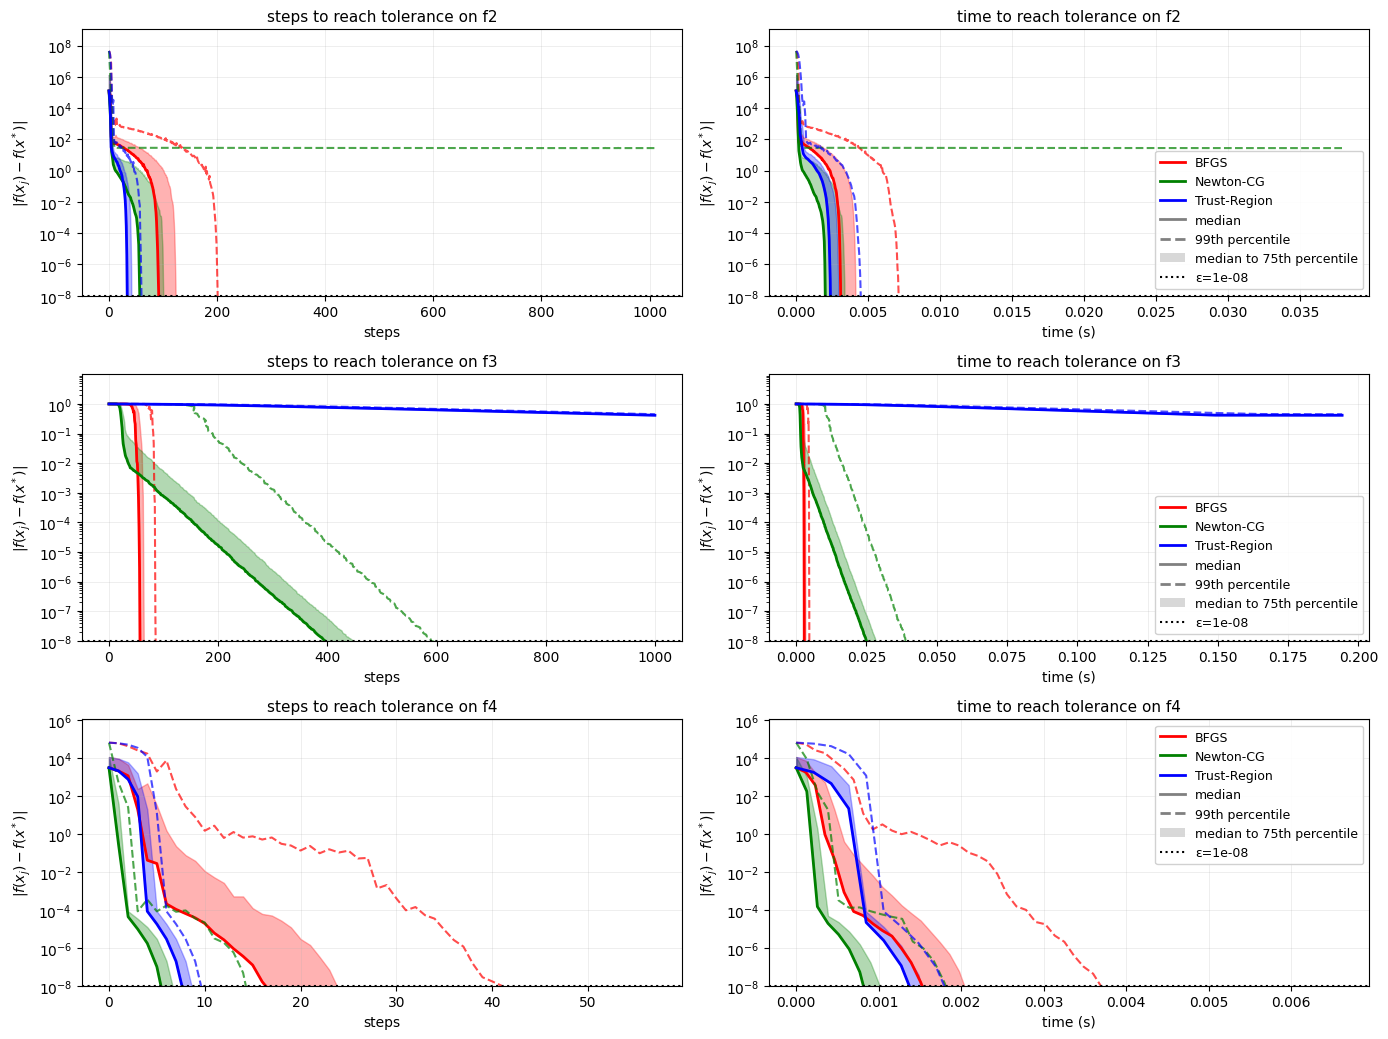
\includegraphics[width=1\textwidth]{plot1.png}
    \caption{
    Median convergence trajectories with 75th percentile band and 99th percentile.
    }
    \label{fig:convergence}
\end{figure}

Figure~\ref{fig:convergence} illustrates the convergence behaviour of the algorithms on three case-study functions selected to expose qualitatively different optimisation challenges.
The Rosenbrock function $f_2$ highlights robustness issues arising from ill-conditioned geometry and strong sensitivity to initialisation.
The transformed ellipsoid function $f_3$ probes algorithm reliability outside globally convex settings, while the attractive-sector function $f_4$ examines the effect of pronounced asymmetry around the optimum.

On the Rosenbrock function $f_2$, all algorithms eventually reach the convergence threshold, but the wide interquartile ranges and heavy-tailed behaviour indicate strong sensitivity to the choice of initial point and limited robustness.
In contrast, the transformed ellipsoid function $f_3$ reveals clear reliability issues, with some algorithms failing to reach the tolerance within the iteration limit.
This behaviour is consistent with the lack of global convexity established in the theoretical analysis.
For the attractive-sector function $f_4$, convergence is achieved more consistently, however, substantial variability in iteration counts highlights differences in algorithm stability and step selection strategies when faced with strong asymmetry.

\begin{table}[h]
\centering
\caption{Percentage of runs that failed to reach $\varepsilon = 10^{-8}$ threshold}
\begin{tabular}{lccccc}
\toprule
Method & f1 & f2 & f3 & f4 & f5 \\
\midrule
BFGS & 0.0\% & 0.0\% & 0.0\% & 0.0\% & 0.0\% \\
Newton-CG & 0.0\% & 16.6\% & 0.0\% & 0.0\% & 0.0\% \\
Trust-Region & 0.0\% & 0.0\% & 100.0\% & 0.0\% & 0.0\% \\
\bottomrule
\end{tabular}
\label{tab:convergence_failures}
\end{table}
The convergence failure analysis shows that BFGS seems to be the most robust algorithm. The trust region method seems to be robust to starting points, but it fails to converge to a good minimum for sum functions, with f3 being an example of this. The Newton method seems to be more sensitive to starting points. 

\subsection{Discussion}
The results demonstrate that algorithm performance depends strongly on the structure of the objective function.
While median convergence rates may suggest good efficiency for certain algorithms, the robustness and reliability analyses reveal important trade-offs.

In particular, algorithms that converge rapidly under favorable conditions may exhibit stagnation or failure for more challenging initializations or non-convex problem structures.
These observations highlight that robustness and reliability are essential considerations in addition to raw efficiency when selecting an optimisation algorithm.
No single algorithm dominates across all tested problem classes, as BFGS is the only algorithm that does not fail to reach the threshold, however, regarding efficiency, it appears to be the slowest one in multiple cases.

\section{Conclusion}
Our analysis reveals that algorithm performance is strongly problem-dependent with no universally superior method. While BFGS demonstrates the most robust behavior, a critical trade-off exists between convergence efficiency and reliability across different problem structures. Practical algorithm selection must prioritize robustness alongside convergence speed, as rapid convergence on favorable problems does not guarantee reliability on non-convex or ill-conditioned objectives.

\end{document}



